\chapter{Kiến thức nền tảng}
\ifpdf
\graphicspath{{Chapter2/Chapter2Figs/PNG/}{Chapter2/Chapter2Figs/PDF/}{Chapter2/Chapter2Figs/}}
\else
\graphicspath{{Chapter2/Chapter2Figs/EPS/}{Chapter2/Chapter2Figs/}}
\fi
\begin{quote}
\textit{Trong chương này sẽ trình bày những kiến thức nền tảng của học tăng cường. Trong phần đầu tiên chúng em sẽ trình bày định nghĩa của các thành phần cơ bản trong học tăng cường. Tiếp đó sẽ đề cập đến mô hình Markov Decision Processes được áp dụng trong việc đánh giá lý thuyết một số thành phần của bài toán học tăng cường. Cùng với đó sẽ trình bày qui trình tổng quát để đánh giá và cải thiện chính sách trong bài toán. Cuối cùng chúng em sẽ trình bày một số phương pháp phổ biến thường đượcAgent áp dụng để đánh giá cũng như cải thiện giúp hệ thông có cách giải tốt hơn cho bài toán trên.}
\end{quote}

\section{Các thành phần cơ bản của học tăng cường}
	\subsection{Agent và môi trường}
	Trong học tăng cường, đối tượng học và đưa ra quyết định được gọi chung là \textit{agent}. Nó tương tác trực tiếp tới một đối tượng được gọi là \textit{môi trường}. Sự tương tác này được diễn ra liên tục. Agent lựa chọn hành động dựa trên những gì nó nhận được từ môi trường. Môi trường cung cấp giá trị điểm thưởng (reward) cho hành động vừa được thực hiện và những quan sát (observation) tiếp theo cho agent. Từ những quan sát này, agent có thể xây dựng ra các \textit{trạng thái} (state) dựa vào đó để ra quyết định chọn hành động với mục tiêu cố gắng đạt được nhiều điểm thưởng nhất.
	
	Cụ thể hơn, agent và môi trường tương tác theo một chuỗi tuần tự các time-steps, $t = 0,1,2,...$. Tại mỗi time step $t$, agent nhận những mô tả trạng thái của môi trường, $\mathit{S_t} \in \mathcal{S}$, với $\mathcal{S}$ là tập các trạng thái có thể có. Dựa vào những mô tả trạng thái nhận được, agent chọn một hành động, $\mathit{A_t} \in \mathcal(\mathit{S_t})$, trong đó $\mathcal(\mathit{S_t})$ là tập các hành động có thể thực hiện tại trạng thái $\mathit{S_t}$. Tại time step sau đó, agent nhận được giá trị điểm thưởng, $\mathit{R_{t+1}} \in \mathbb{R}$, cùng với trạng thái tiếp theo $\mathit{S_{t+1}}$ Quá trình tương tác giữa agent và môi trường được mô tả trong hình \ref{AgentEnvironment}
		
	\begin{figure}
		\centering
		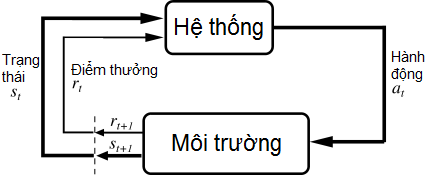
\includegraphics[width=\textwidth]{AgentEnvironment}
		\caption{Quá trình tương tác giữa hệ thông và môi trường}
		\label{AgentEnvironment}
	\end{figure}
	
	Các thành phần của agent gồm có:
	\begin{itemize}
		\item \textbf{Chính sách}. Chính sách, $\pi$, xác định khả năng chọn một hành động khi agent nhận được một trạng thái $s$. Chính xác tại time step $t$ được xác định $\pi_t(a|s) = \mathbb{P}[\mathit{A_t} = a|\mathit{S_t} = s]$. Để đạt được mục tiêu được nhiều điểm thưởng nhất, agent cần có một\textit{chính sách} chọn lựa hành động phù hợp mỗi khi gặp một trạng thái. Những phương pháp học tăng cường thường tập trung thay đổi các chính sách của agent sao cho đạt được kết quả tốt trong thực nghiệm.
		\item \textbf{Hàm giá trị}. Hầu hết các thuật toán học tăng cường đầu tập trung đánh giá những \textit{hàm giá trị}, các hàm này đánh giá một trạng thái hoặc hành động là tốt như thế nào cho agent thông qua việc ước lượng điểm thưởng nhận được ở tương lai. Thông thường, giá trị của một trạng thái $s$, dưới một chính sách $\pi$  được ký hiệu $v_{\pi}(s)$ là lượng điểm thưởng kỳ vọng nhận được bắt đầu từ trạng thái $s$ về sau.
		\item \textbf{Mô hình}. Agent xây dựng mô hình cho riêng mình để mô phỏng môi trường và dự doán các thông tin của môi trường trong tương lai.
	\end{itemize}	
	
	\subsection{Returns}
	Return $\mathit{G_t}$ xác định lượng điểm thưởng mà agent nhận được kể từ thời điểm time step $t$ đến tương lai. Return thường được xác định bằng nhiều hàm khác nhau, trong đó hàm đơn giản nhất xác định return bằng tổng các điểm thưởng có thể nhận được. Nó có dạng như sau:
	$$\mathit{G_t} = \mathit{R_{t+1}} + \mathit{R_{t+2}} + ... + \mathit{R_{T}}$$
	ở đây $T$ là time step cuối cùng.
	
	Mặt khác, return cũng có thể được xác định bằng tổng điểm thưởng đã bị discount qua từng time step. Nó được định nghĩa như sau:
	$$\mathit{G_t} = \mathit{R_{t+1}} + \gamma\mathit{R_{t+2}} + \gamma^{2}\mathit{R_{t+3}}... + \gamma^{T-1}\mathit{R_{T}} = \sum_{k=0}^{\infty}\gamma^{k}\mathit{R_{t+k+1}}$$
	Trong đó $\gamma$ là một hệ số với giá trị $0\leqslant \gamma \leqslant 1$. $\gamma$ cũng được gọi là tỉ lệ discount. Tỉ lệ này xác định độ tin tưởng của agent vào giá trị điểm thưởng ở tương lai. Khi $\gamma \to 1$, agent có su hướng quan tâm đến giá trị điểm thưởng tương lai càng nhiều. Đặc biệt với $\gamma = 0$, khi đó agent chỉ quan tâm giá trị điểm thưởng ở hiện tại mà bỏ qua những giá trị điểm thưởng ở tương lai.
	
	Trong thực nghiệm, việc tương tác giữa agent và môi trường có thể được phân chia thành những chuỗi con. Chúng được gọi là những \textit{episode}. [TODO]
	
	
\section{Mô hình Markov Decision Processes}
%	\begin{itemize}
%			\item Các thành phần MDP
%			\item Ví dụ cho mô hình MDP
%			\item Phương trình Bellman
%			\item Qui trình đánh giá chính sách: Kỹ thuật qui hoạch động
%			\item Qui trình cải thiện chính động: Kỹ thuật qui hoạch động
%	\end{itemize}
	\subsection{Định nghĩa mô hình Markov Decision Processes}
	Mô hình Markov Decision Processes (MDP) được sử dụng để mô hình hóa bài toán học tăng cường một cách có hình thức. Cụ thể, MDP là một bộ bao gồm 5 thành phần $<\mathcal{S, A, P, R, \gamma}>$ trong đó:
		\begin{itemize}
			\item $\mathcal{S}$: tập trạng thái hữu hạn có thể có của môi trường.
			\item $\mathcal{A}$: tập những hành động hữu hạn mà hệ thống có thể thực hiện để tương tác với môi trường.
			\item $\gamma$: Hệ số có giá trị thỏa $0\leqslant \gamma \leqslant 1$ thể hiện mức độ tin tưởng về giá trị điểm thưởng nhận được ở tương lai.
			\item $\mathcal{P}$: ma trận xác suất chuyển trạng thái. Trong đó $\mathcal{P}_{ss'}^{a}$ là xác suất chuyển đến trạng thái $s'$ khi hệ thống đang ở trạng thái $s$ và thực hiện hành động $a$.
				\begin{equation}
					\mathcal{P}_{ss'}^{a} = \mathbb{P}[\mathit{S_{t+1}} = s' |\mathit{S_{t}} = s, \mathit{A_{t}} = a]
				\end{equation}
			\item $\mathcal{R}$: ma trận điểm thưởng theo từng bộ (trạng thái, hành động). $\mathcal{R}_{s}^a$ là kỳ vọng giá trị điểm thưởng nhận được khi hệ thống thực hiện hành động $a$ ở trạng thái $s$.
				\begin{equation}
					\mathcal{R}_{s}^a = \mathbb{E}[\mathit{R_{t}} | \mathit{S_{t}} = s, \mathit{A_{t}} = a]
				\end{equation}				
		\end{itemize}
	
	\textbf{Ví dụ: Mô hình MDP trong robot thu gom} Công việc của robot này là thu lượm những lon soda đã được uống hết trong văn phòng. Nó có những cảm biến để xác định những lon soda này, bánh xe và cánh tay để di chuyển và gắp nhặt những lon này bỏ vào thùng. Robot hoạt động bằng pin sạc. Hệ thống điều khiển của robot có chức năng tiếp nhận những thông tin từ cảm biến từ đó điểu khiển bánh xe và cánh tay. Trong ví dụ, chúng em chỉ xét dựa trên mức độ pin hiện tại robot nên quyết định tìm kiếm những lon soda như thế nào? Robot có thể có ba quyết định (1) thực hiện tìm kiếm một lon soda, (2) đứng yên và đợi người khác mang lon soda đến cho nó, (3) quay trở lại nơi sạc pin. Trạng thái của môi trường được xác định là trạng thái của pin hiện tại của robot. Cách tốt nhất để tìm kiếm những lon soda là robot thực hiện hành động tìm kiếm, nhưng việc này sẽ làm giảm dung lượng của pin.

\section{Những phương pháp đánh giá và cải thiện chính sách}
	\begin{itemize}
		\item Dẫn nhập: Trên thực tế ta không có thông tin về môi trường
		\item Qui trình đánh giá chính sách
			\begin{itemize}
				\item[+] Dựa trên hàm giá trị trạng thái: Monte-Carlo, TD(0), n-step TD, TD($\lambda$)
				\item[+] Dựa trên hàm giá trị hành động: Monte-Carlo, Sarsa(0), n-step Sarsa, Sarsa($\lambda$)
			\end{itemize}
		\item Qui trình cải thiện chính sách: Phương pháp greedy
	\end{itemize}
	
